\documentclass{article}

\usepackage{amsfonts}
\usepackage{graphicx}
\usepackage{amssymb}
\usepackage{amsmath}
\usepackage{listings}


\DeclareMathOperator{\sech}{sech}
\newcommand{\NN}{\mathbb{N}}
\newcommand{\RR}{\mathbb{R}}
\newcommand{\QQ}{\mathbb{Q}}
\newcommand{\ZZ}{\mathbb{Z}}
\newcommand{\dV}{\;\mathrm{d}V}
\newcommand{\dA}{\;\mathrm{d}A}
\newcommand{\dx}{\;\mathrm{d}x}
\newcommand{\dy}{\;\mathrm{d}y}
\newcommand{\dz}{\;\mathrm{d}z}
\newcommand{\cA}{\mathcal{A}}
\newcommand{\Bb}{\mathcal{B}}
\newcommand{\Ww}{\mathcal{W}}
\newcommand{\Dd}{\mathcal{D}}
\newcommand{\Ss}{\mathcal{S}}
\newcommand{\Ee}{\mathcal{E}}
\DeclareMathOperator{\im}{im}


\setlength\parindent{18pt}

\begin{document}

Textbook Section 7.1:

1) For $f(t) = t$, the Laplace transform becomes:
\[F(s) = \int_{0}^{\infty} e^{-st} t dt\]

which computes to:
\[F(s) = \frac{1}{s^2}\]

The result is valid for $Re(s) > 0$.

6) For $f(t) = \sin^2(t)$, the Laplace transform becomes:
\[F(S) = \int_{0}^{\infty} e^{-st} \sin^2(t) dt\]

We can simplify this using the trig identity:
\[\sin^2(t) = \frac{1 - \cos(2t)}{2}\]

So, the Laplace transform becomes:
\[F(s) = \frac{1}{2} \int_{0}^{\infty} e^{-st} [1 - \cos(2t)] dt\]

which computes to:
\[F(s) = \frac{2}{s(s^2 + 4)}\]

This result is valid for $Re(s) > 0$.

20) The Laplace transform of $f(t) = e^{a t}$ is $\frac{1}{s - a}$ for $s > a$.
For our case, $a = 1$.

For integration by parts, $u(t) = t$, $v'(t) = e^t$.

We know that the Laplace transform of $t^n$ is $\frac{n!}{s^{n+1}}$ for $n \geq 0$ and $s > 0$.
For $n = 1$, the Laplace transform is $\frac{1}{s^2}$. We can use the linearity of the Laplace
transform to multiply this by the transform of $e^t$, which is $\frac{1}{s-1}$ for $s > 1$.

\[L\{te^t\} = L\{t\} \cdot L\{e^t\}\]
\[L\{te^t\} = \frac{1}{s^2} \cdot \frac{1}{s-1}\]

So, $F(s) = \frac{1}{s^2(s-1)}$.

30) Let's factor the denominator $\frac{9+s}{4-s^2}$ using partial fractions.
The partial fraction decomposition is $\frac{7}{4(s+2)} - \frac{11}{4(s-2)}$.

So, the inverse Laplace transform is:
\[L^{-1}\{\frac{7}{4(s+2)}\} - L^{-1}\{\frac{11}{4(s-2)}\}\]

Using the table, this translates to:
\[\frac{7}{4} e^{-2t} - \frac{11}{4} e^{2t}\]

Hence the inverse Laplace transform is:
\[f(t) = \frac{7}{4} e^{-2t} - \frac{11}{4} e^{2t}\]


Textbook Section 7.2:

1) We start by taking the Laplace transform of each term in the differential equation.

\[L\{x''\} = s^2 X(s) - sx(0) - x'(0)\]

Plugging in initial conditions, we get:
\[L\{x''\} = s^2 X(s) - 5s\]

By applying the Laplace transform to both sides of the equation, we get:
\[s^2 X(s) - 5s + 4 X(s) = 0\]

Now, solve for $X(s)$.
\[X(s) = \frac{5s}{s^2 + 4}\]

To get $x(t)$, we have to compute the inverse Laplace transform of $X(s)$.
$X(s)$ corresponds to $5 \cos(2t)$ in the time domain.

So, the initial value problem is:
\[x(t) = 5 \cos(2t)\]

4) Doing the same process as above gives us the Laplace transform of the differential equation as:
\[s^2 X(s) - 2s + 3 + 8(s X(s) - 2) + 15 X(s) = 0\]

Then we solve for $X(s)$.
\[X(s) = \frac{2s - 13}{(s+3)(s+5)}\]

Then we have to take the partial fraction decomposition of $X(s)$.
\[X(s) = \frac{23}{2(s+5)} - \frac{19}{2(s+3)}\]

Then we take the inverse Laplace transform:
\[x(t) = L^{-1}\{\frac{23}{2(s+5)}\} - L^{-1}\{\frac{19}{2(s+3)}\}\]
\[x(t) = \frac{23}{2} e^{-5t} - \frac{19}{2} e^{-3t}\]

20) The partial fraction decomposition of $\frac{2s+1}{s(s^2+9)}$ is
$-\frac{s-18}{9(s^2 + 9)} + \frac{1}{9s}$

\[L^{-1}\{\frac{1}{s}\} = 1\]
\[L^{-1}\{\frac{s}{s^2 + 9}\} = \cos(3t)\]
\[L^{-1}\{\frac{2}{s^2 + 9}\} = \frac{2}{3} \sin(3t)\]

Putting this together using the properties of Theorem 2 gives:
\[f(t) = -\frac{1}{9} \int_{0}^{t} \cos(3 \tau) d \tau + \frac{2}{3} \int_{0}^{t} \sin(3 \tau) d \tau + \frac{1}{9}\]

So, we get that:
\[f(t) = -\frac{1}{27} \sin(3t) - \frac{2}{9} \cos(3t) + \frac{1}{9}\]


Textbook Section 7.3:

3) The Laplace transform of $\sin(bt)$ is $\frac{b}{s^2 + b^2}$. So the Laplace
transform of $\sin(3 \pi t)$ is $\frac{3 \pi}{s^2 + (3 \pi)^2}$.
Using the translation theorem, we replace $s$ with $s + 2$.

So,
\[L\{e^{-2t} \sin(3 \pi t)\} = \frac{3 \pi}{(s+2)^2 + (3 \pi)^2}\]

8) We will first complete the square in the denominator.
Completing the square for $s^2 + 4s + 5$ gives $s^2 + 4s + 4$.

We can rewrite $F(s)$ as:
\[F(s) = \frac{s+2}{(s+2)^2 + 1}\]

Using the translation theorem,
\[f(t) = L^{-1}\{\frac{s+2}{(s+2)^2 + 1}\} = e^{2t} \cos(t)\]

19) Let $s^2 = x$. Then the denominator factors into $(s^2 + 1)(s^2 + 4)$.
The partial fraction decomposition of $F(s)$ is:
\[F(s) = \frac{2(s+2)}{3(s^2 + 4)} - \frac{2s+1}{3(s^2 + 1)}\]

Using a table, we find that:
\[\frac{2}{3} \cos(2t) + \frac{2}{3} \sin(2t) - \frac{2}{3} \cos(t) - \frac{1}{3} \sin(t)\]

30)
\[L\{x''\} = s^2 X(s)\]
\[L\{x'\} = s X(s)\]

Applying the Laplace transform to the entire differential equation gives:
\[(s^2 + 4s + 8) X(s) = \frac{1}{s+1}\]

Solve for $X(s)$.
\[X(s) = \frac{1}{(s+1)(s^2 + 4s + 8)}\]

Taking the partial fraction, we get:
\[X(s) = -\frac{s+3}{5(s^2 + 4s + 8)} + \frac{1}{5(s+1)}\]

\[s^2 + 4s + 8 = (s+2)^2 + 4\]

We eventually get that:
\[x(t) = \frac{1}{5} e^{-t} - \frac{1}{10} e^{-2t} \sin(2t) - \frac{1}{5} e^{-2t} \cos(2t)\]


Textbook Section 7.4:

5)
\[(f * g)(t) = \int_{0}^{t} e^{a \tau} e^{a (t - \tau)} d \tau\]

Which is equal to:
\[(f * g)(t) = e^{at} t\]

So, $(f*f)(t) = e^{at} t$.

10)
\[F(s) = \frac{1}{s^2} \cdot \frac{1}{s^2 + k^2}\]

\[f(t) * g(t) = t * \frac{1}{k} \sin(kt)\]

Doing some algebra and computation (of the convolution) gives:
\[f(t) = \frac{kt - \sin(kt)}{K^3}\]


19) The given function can be considered the integral of $\sin(t)$ from $0$ to
$t$ divided by $t$. We know the Laplace transform of $\sin(t)$ is $\frac{1}{s^2 + 1}$.

According to Theorem 3, the Laplace transform of $\frac{\sin(t)}{t}$ is the integral of
$\frac{1}{s^2 + 1}$ with respect to $s$ from $0$ to $\infty$.

Calculating this gives us:
\[F(s) = -arctan(s) + \frac{\pi}{2}\]


Textbook Section 7.5:

1) Using the second shifting (delay theorem), we get that:
\[f(t) = (t-3) u(t-3)\]

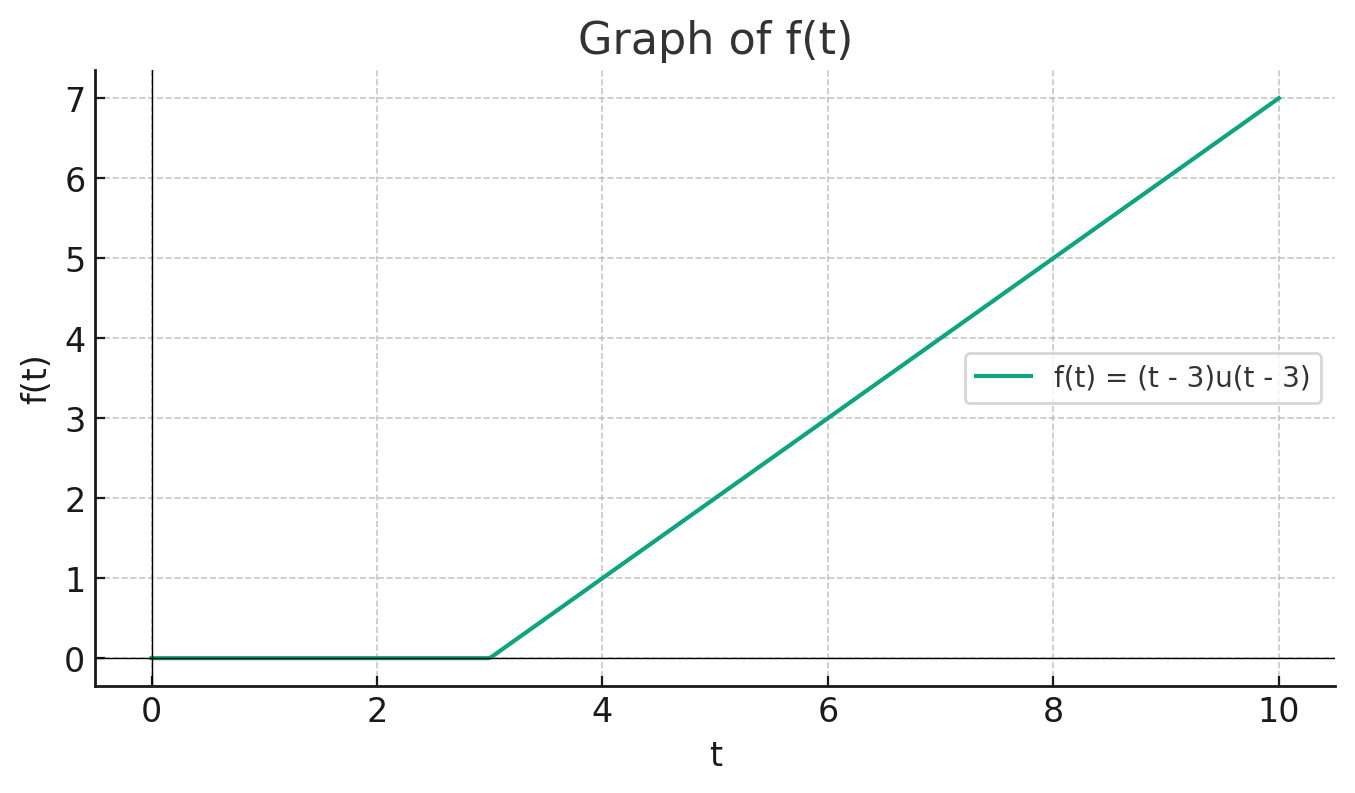
\includegraphics[width=\linewidth]{7_5_1}

6) Applying the first shifting theorem, we get that:
\[f(t) = \cos(\pi(t-1)) u(t-1)\]

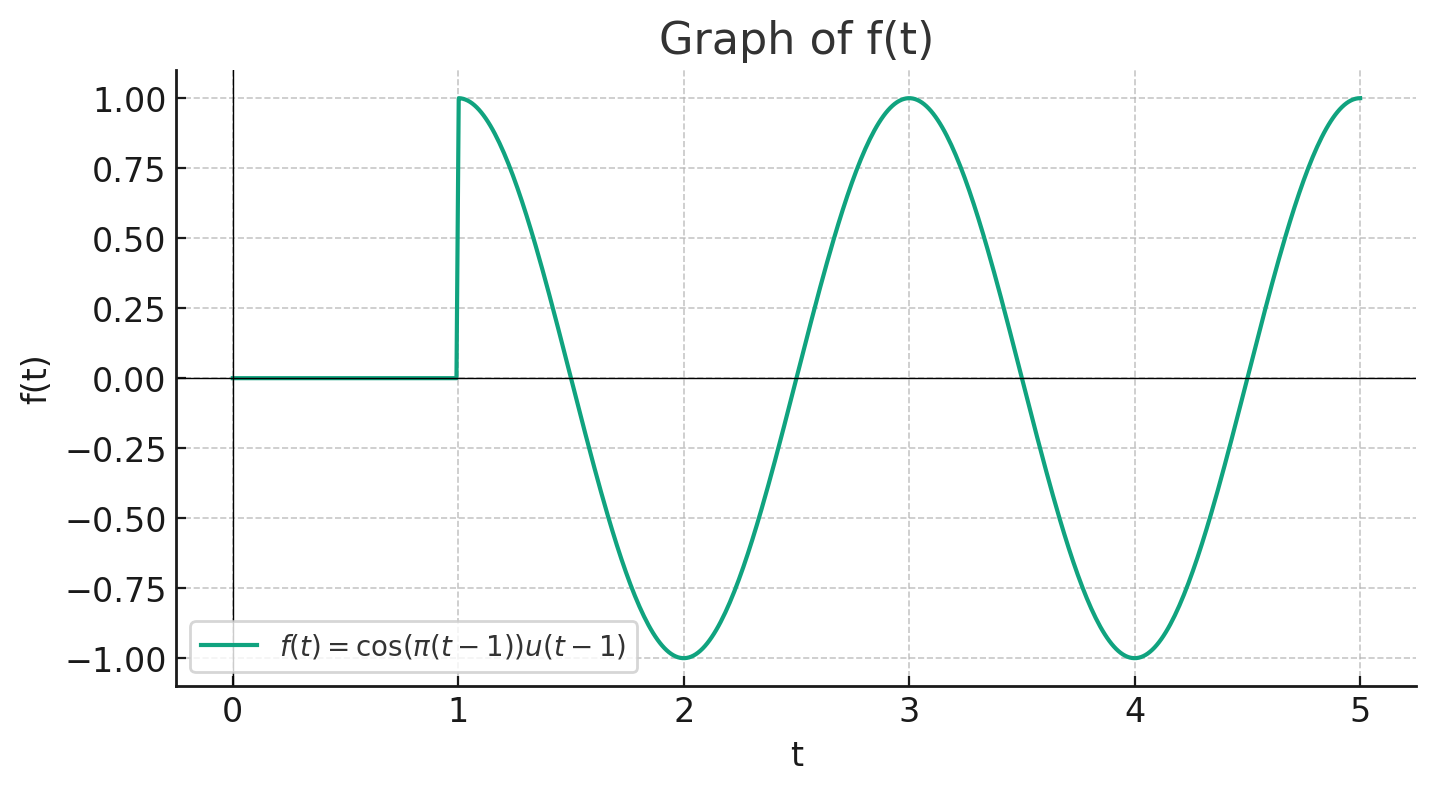
\includegraphics[width=\linewidth]{7_5_6}

21) We can write:
\[L\{f(t)\} = L\{tu(t) - tu(t-1)\} + L\{2u(t-1) - tu(t-1) - 2u(t-2) + tu(t-2)\}\]
Using the first shifting theorem, we get that:
\[L\{f(t)\} = \frac{e^{2s} - 2e^s + 1}{s^2} e^{-2s}\]


Textbook Section 7.6:

1)
\[L\{x'\} = sX(s)\]
\[L\{x''\} = s^2 X(s)\]
Applying the Laplace transform to the entire differential equation, we get:
\[(s^2 + 4) X(s) = 1\]
\[X(s) = \frac{1}{s^2 + 4}\]
\[x(t) = \frac{1}{2} \sin(2t)\]

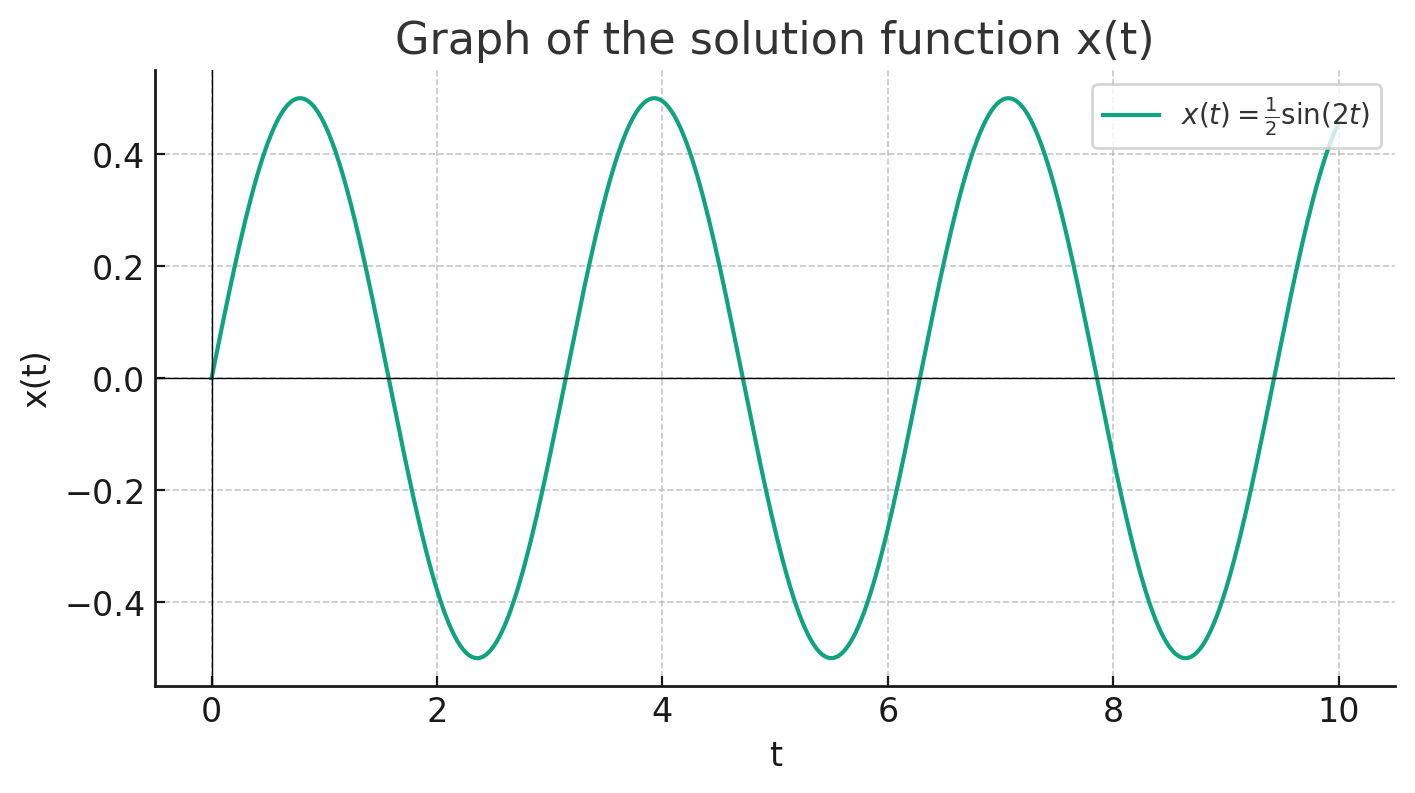
\includegraphics[width=\linewidth]{7_6_1}

\end{document}
